\chapter{Literature Review}

\section{Introduction}
% This introduction is pretty poor, probably best to rewrite once the rest is finished
In this chapter an overview is given of the existing literature as well as an overview of topics that are relevant to this project. The chapter is split into two sections. The first section gives a review of Model Driven Engineering and tools that can be used for implementation. The second section investigates software testing methods and ways of assessing the quality of software tests.

\section{Model Driven Engineering}

\subsection{Introduction}
% The Oxford English dictionary defines Model Driven Engineering as... just kidding
Model Driven Engineering is a development methodology that aims to reduce the amount of time spent on projects, as well as increasing the consistency and quality of the item or system under development. Model driven engineering can be useful when developing software. A model of the software architecture can be created, and from that a code generation tool can be run. Assuming that the model is correct, human typing errors are avoided and precious development time can be spent on more important aspects than hunting for trivial bugs. Maintenance is also easier, as changes can be applied to the model, and the updated code will be generated automatically from the model. Finally, the code generation can be to a multitude of languages and platforms, further reducing time spent on development \cite{mdseLano}.

%Model Driven Engineering is a development methodology that aims to reduce the amount of time spent on code development by building models that can be transformed and used to generate code automatically. Bugs that would normally be in code (through developer error) will no longer be present, as all the code has been generated automatically from a model. Of course this assumes that the model is correct in the first place. Cross-platform implementation overheads are also reduced. The model can remain the same for all platforms, and only the model-to-code program has to be modified for different target platforms. \citep{mdseLano}.

In the 1980's there was a software quality crisis that lead to the search for alternative approaches to developing software. Model Driven Engineering is one solution that was of interest at the time as it provided a way to visually represent a system architecture, and from that generate code automatically. However, the return on investment that companies were expecting from model driven engineering was far too high, causing much disappointment and disillusionment, and for a while the concept was sidelined. More recently, the Object Managment Group (OMG) have promoted and developed a Unified Modeling Language (UML), and tools such as Epsilon have further promoted the use of MDE \citep{mdeHistory}.  \citet{brambillaBook} believes that Model Driven Engineering is now past the `trough of disillusionment' and into the `slope of enlightenment' (see Figure \ref{mde_pos}). By this they mean that new technologies often make many promises that they ultimately cannot fulfil, which is represented by the peak of inflated expectations on the graph. From the disappointment that comes with broken promises, people become disillusioned with the technology and people tend to avoid using it, as shown by the trough of disillusionment. Researchers continue to work on improving and maturing the technology, which is represented by the slope of enlightenment. \\

\begin{figure}
\begin{minipage}{0.5\textwidth}
	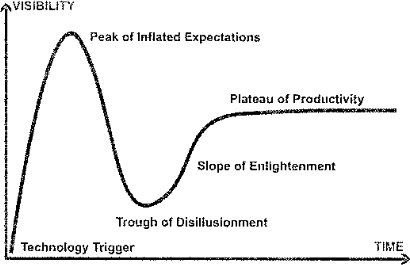
\includegraphics[width=0.9\linewidth]{figures/mde_pos.jpg}
\caption{The technology hype cycle according to \citet{brambillaBook}}
\label{mde_pos}
\end{minipage}
\begin{minipage}{0.49\textwidth}
	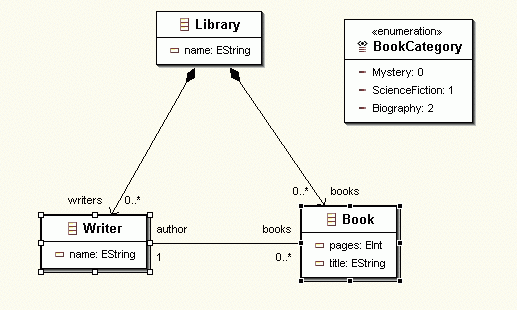
\includegraphics[width=0.9\linewidth]{figures/sample_model.png}
\caption{A sample model \citep{sampleModel}}
%TODO: Create my own model to sample here?
\label{uml_sample}
\end{minipage}
\end{figure}

\subsection{Model}

A model is a representation of something that abstracts away many details that are not necessary for its use \citep{brambillaBook}. For example, the Utah Teapot \citep{Crow:1987:OT} is a model of a teapot that is rendered by a 3D engine. However, many aspects of the teapot are not considered in its model, as they are not necessary for a simple render. An example is that the lid is not a removable component, because for the purpose of rendering the teapot, the lid never has to be removed. Another example is that the only physical property of the teapot that will be included in the model is its finish (texture), so that lighting and reflection can be calculated. Other details such as its weight will not be included in the model, because it is not necessary.

UML (Unified Modeling Language) is a language that is designed specifically for representing models visually. It is ideal for object-oriented design, as it represents classes with boxes and associations between classes with lines. Within the boxes there are definitions of the classes, methods and fields. In Figure \ref{uml_sample}, book is a class that has the properties pages and title. The diagram also shows that there is the association author between a writer object and a book object.

\subsection{Metamodels}
To have a modeling language, there must be a specification of that language that defines the valid syntax, constraints etc. In the case of UML, the Object Management Group provide a detailed specification \citep{umlSpec} of the language, and we can check that any diagram is a UML diagram by checking that it complies with the UML specification.
%Concrete, Abstract and semantic sections...
A metamodel is the specification of a modeling language, in the form of a model \citep{brambillaBook}. A metamodel could be represented visually or textually (as can a model), depending on the specification of the metamodeling language. As with many aspects of computer science, the metamodel is just another layer of abstraction, and we can continue to abstract to higher and higher levels. A metametamodel (known as M3) will define the specification of a metamodeling language, and the abstraction can continue as far as is required.

Going back to the example of The Utah Teapot, the metamodel in this case may define that the teapot is made up from interconnected polygons, and specify that each polygon has a location and size given in 3D space. 

\subsubsection{Abstract and Concrete Syntax}

When building a metamodel, both the abstract and concrete syntax must be defined. The abstract syntax of a language is a definition of how the language components interact. For an OO language, the abstract synatax would specify that a class can inherit the properties of another class, that a class must have a constructor, and that a class must be given a name. How these requirements are met by the user is specified by the concrete syntax. The concrete syntax for allowing class inheritance would state that the colon symbol must be used after the class name:

\begin{lstlisting}
class NewClass : ParentClass
\end{lstlisting}

The concrete syntax does not necessarily need to be textual. To build a modeling language you require a metamodel, which is the abstract syntax. You also require a way to visually display the model. The concrete syntax could state that a class is represented as a rectangle with the name of the class in the middle, and that to show inheritence the NewClass must have an arrow coming out of it that goes to the ParentClass that it is inheriting from.

\begin{figure}[h]
\begin{center}
	\includedot[scale=0.5]{figures/concrete_syntax}
	\label{concreteSyntaxFigure}
	\caption{Concrete Syntax example for a modeling language}
\end{center}
\end{figure}

\subsection{Epsilon}
With the theory of model driven engineering covered, the focus will now turn to covering the tools that can be used in model driven engineering, and that will be used in this project.

Epsilon is a suite of languages and tools that provide all the necessary components to build and manipulate models. Epsilon stands for \textbf{E}xtensible \textbf{P}latform of Integrated \textbf{L}anguages for M\textbf{O}del Ma\textbf{N}agement \citep{epsilonWebsite}. It is part of the Eclipse Modeling Project \citep{ecliplseModelingProjectSite}, and includes tools for each of its languages that integrate with Eclipse. From the Epsilon Website \citep{epsilonWebsite}, the languages that are provided by Epsilon are:

\begin{description}
\item[EOL] Epsilon Object Language is an expression language that is used to create, query and model EMF models. All other languages included in Epsilon are based on EOL \citep{epsilonBook}
\item[ETL] Epsilon Transformation Language is a model-to-model transformation language.
\item[EVL] Epsilon Validation Language is a model constraint language.
\item[EGL] Epsilon Generation Language is a model-to-text generation language that can be used to generate code from models.
\item[EWL] Epsilon Wizard Language is similar to ETL, except that ETL performs batch operations whereas EWL works with in-place model transformations based on user selections.
\item[ECL] Epsilon Comparison Language is a model comparison language.
\item[EML] Epsilon Merging Language is used to merge models of diverse metamodels.
\item[Epsilon Flock] A rule based transformation language.
\end{description}

For each of these languages Epsilon provides development tools for use in Eclipse, as well as interpreters for each of the languages. As well, ANT workflows are provided which are a way of automating tasks in a sequential manner \citep{epsilonBook}.

\subsection{EUnit}
EUnit is a unit testing framework that is included with Epsilon \citep{epsilonWebsite}. It allows systematic testing of model transformations by providing tools that can be used for checking that the output of model transformations meet certain requirements. \citep{epsilonBook} EUnit allows for different inputs and models, and could be considered as a JUnit for models. Notably, EUnit does not include test coverage analysis, which is the focus of this project.

\subsection{Graphical Modeling Framework}

The Eclipse graphical modeling framework (GMF) is part of the Eclipse Graphical Modeling Project \citep{gmpSite}. The Eclipse Wiki \cite{gmpFAQ} states that:

\begin{quote} Using GMF, you can produce graphical editors for Eclipse. For example, a UML modeling tool, workflow editor, etc. Basically, a graphical editing surface for any domain model in EMF you would like. \end{quote}

To create these graphical editors, GMF requires 6 different files \citep{gmfIntro}, including a metamodel of the models that the graphical editor will be used to create, graphics that will be used for representing models, and the tools that can be used to manipulate models.

\subsection{EuGENia}
EuGENia is one of the tools that is included with Epsilon. EuGENia takes an Ecore metamodel specification and generates a GMF editor \citep{eugeniaSite}. The purpose of EuGENia, as taken from its website, is to `shield you from the complexity of GMF and lower the entrance barrier for creating your first GMF editor.' \citep{eugeniaSite} From the code listed in Appendix \ref{App:SampleEuGENia}, the model editor shown in Figure \ref{sampleGmf} is generated by EuGENia.

\begin{figure}
\begin{center}
	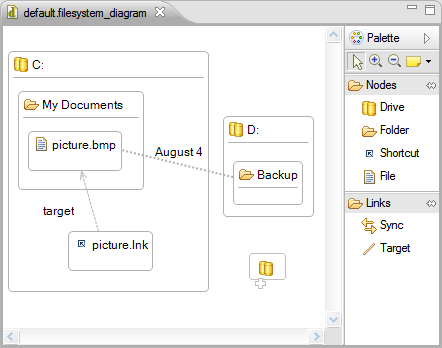
\includegraphics[width=3in]{figures/gmfeditor.png}
\end{center}
\caption{A sample gmf editor generated by EuGENia \citep{eugeniaSite}}
\label{sampleGmf}
\end{figure}

The generated editor provides the objects shown on the right hand side of Figure \ref{sampleGmf}. These objects are then dragged to the left hand section of the editor by the user, where associations between objects can be intuitively created.

\subsection{Model Transformation Testing}

To bring model-driven-engineering out of the `trough of disillusionment' it has been necessary to perform testing on model transformations before they are deployed to users. Much research has been done in this area, and \citet{mttBarriers} describe the three stages to model transformation testing:

\begin{enumerate}
	\item Generate test data: As with any type of test, there needs to be some input to the system. In this case it will be a set of models that are to be transformed. These models will conform to the metamodel that specifies input to the model transformation, and will either be manually created by the tester, or automatically generated in the form of graphs of metamodel instances \citep{mttBarriers}.
	\item Define test adequacy criteria: For any modeling language beyond the very basic there will be a very large number of possible inputs. This rules out running every possible model through the transformer in to test it as it would take too long. Instead a test adequacy criteria must be defined that allows the effective seletion of test models. According to \citet{mttBarriers}, there is no well-defined criteria for model transformation testing.
	\item Construct an oracle: The oracle gets the output of the system and determines if it is correct (based on the test input model).
\end{enumerate}

\citet{fleureyMTInputs} propose a general framework for assessing the quality of model transformations. Their paper begins by discussing the possibility of finding `partitions' of the transformation's input meta-model. A partition is where the model could be one of a range of values, so for example if the metamodel specifies a boolean, there is a partition as the boolean could be either true or false. With these partitions, we could check that the input test set covers each possible combination of partitions. \citet{fleureyMTInputs} then go on to state why this isn't necessarily the most useful approach: first the complexity rises quickly with each additional partition. Secondly, some of combinations of partitions will not be relevant for testing, and the tester would have to find these and remove them. Finally, some relevant combinations could be missing. Generating every single combination of partition will `not ensure the existence of more than one composite state', they state.

What \citet{fleureyMTInputs} propose is the idea of model and object fragments that `define specific combinations of ranges for properties that should be covered by test models'. Their paper suggests that one of the more important aspects of model transformation testing is ensuring that input models cover the correct criteria - that they thoroughly test the transformation, while avoiding having many very similar inputs that don't test anything that has not already been tested by another input.

The oracle can be difficult to create for any complex model transformation. \citet{mttOracleIssue} propose six ways that an oracle could be implemented for model transformation testing:

\begin{enumerate}
	\item Compare the output to a reference model (i.e. the expected output model for the particular input). Unfortunately this requires that the tester has to create the expected models for each test. For a large test set this could be incredibly time consuming.
	\item Perform an inverse transformation on the output. This would give the original input model, if the model transformation was correct. This requires that the tester implement a reverse transformation, and also requires that the transformation is an injective function (i.e. a function that preserves distinctness). According to \citet{mttOracleIssue}, this is unfortunately unlikely.
	\item Compare the output with that from a reference model transformation. This reference model transformation can produce the reference model from the test model. 
	\item A generic contract is a list of constraints on the output of the model transformation based on the input. Once the model transformation has completed, the output model is checked against the constraints defined in the generic contract.
	\item The tester could provide a list of assertions in OCL (or EVL) that can be checked on the output model. Not every detail about the output model must be provided. Doing so would be a waste of time as providing the expected output model would be quicker.
	\item Model snippets could be provided by the tester. Each snippet is associated with a cardinality and logical operator so that the expected number of occurrences of each snippet can be calculated. The oracle would check that the expected number of each snippet appears in the output. 
\end{enumerate}

\section{Quality of Software Testing}
\subsection{Introduction}

Users expect software to work without issues, and so when a bug is encountered, the user will at best be annoyed. At worst, the bug may be in a critical piece of software that the failure of which could result in the loss of millions of dollars, or even human lives. The need for the testing of software before it is released then hardly requires justification. But how do we know when software has been tested thoroughly enough? This section will look at different approaches to determining the quality of a test suite. 

\subsection{The Need for Test Quality Metrics}

To try and further justify the need for thorough software tests, I discuss two rather serious cases where software has failed where testing should have caught the bugs.

The Ariane 5 rocket cost \$7 billion to develop, and so of course any software on board would have had test suites to ensure that it did not fail. Unfortunately in 1996, 37 seconds after launch, \$500 million of rocket and cargo exploded because of an integer overflow \citep{ariane5}. Despite having software tests, the tests were clearly insufficient as they did not find the integer overflow problem prior to the software being put into use. The software turned the rocket in the wrong direction, and to minimise the risk of fatalities the decision was quickly made to destruct the rocket. Thankfully there was no-one on board, and no-one on the ground was injured.

In 1991 though, a software error lead to the death of 28 people. The Patriot missile system was supposed to track incoming ballistic missiles and launch a rocket to destroy them before they hit their target \citep{patriotMissile}. In one instance the system lost track of an incoming missile and decided that it must have been a false reading, and so no rocket was launched. The incoming missile hit a US barrack, killing 28 American soldiers. The software for the Patriot missile lost time after being switched on for too long, meaning that it was looking in the wrong place for the incoming missile. There is no doubt that the system was tested before it was deployed, but clearly testing was not comprehensive enough. 

The final example is more recent. In February 2014 Apple issued a security update that fixed a bug in their SSL software. The bug was contained in the code in Figure \ref{fig:AppleBug}. Notice that there is a duplicated \verb|goto| statement, but because no braces were used on the above \verb|if| statement, the duplicated statement is not conditional, and will be always executed. This is another case of insufficient testing. In this particular case, some analysis of which lines of code are executed by the test suite (i.e. line coverage analysis) would have shown that the final if statement in that block of code was never executed, because the above goto is always called.

\begin{figure}
	\centering
	%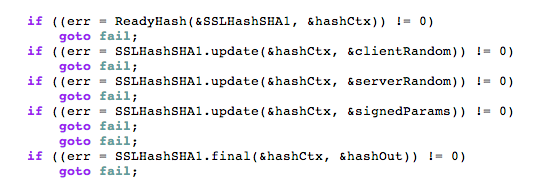
\includegraphics[scale=0.4]{figures/appleBug.png}
	\lstinputlisting[language=java]{code/appleBug.java}
	\caption{Apple's SSL bug}
	\label{fig:AppleBug}
\end{figure}

% Section about testing requrements
\subsection{Coverage}

Test sets have a \emph{coverage criterion} that measures how good a collection of sets is \citep{softwareTestingIntro}. According to \citet{softwareTestingIntro}, coverage is defined as:

\begin{quote} Given a set of test requirements $TR$ for a coverage criterion $C$, a test set $T$ satisfies $C$ if and only if for every test requirement $tr$ in $TR$, at least one test $t$ in $T$ exists such that $t$ satisfies $tr$ \end{quote}

In addition to coverage, coverage level is also defined by \citep{softwareTestingIntro} as:

\begin{quote}Given a set of test requirements $TR$ and a test set $T$, the coverage level is simply the ratio of the number of test requirements satisfied by $T$ to the size of $TR$\end{quote}.

There are different approaches to determining the test coverage level of a program. Below I discuss each of these.

\subsection{Statement Coverage}

Arguably the most simple approach to determining the quality of a test set is to analyse the number of lines of code that execute when the tests are run. If all lines of code are executed at least once when all tests have been run, then statement coverage is said to be 100\% \citep{softwareTestingIntro}.

While simple to implement, line coverage suffers from a serious downfall. In most programming languages it is perfectly valid to have as many operations on one line as the developer chooses. In an extreme case it would be possible for the developer to have the whole program on one line. A contrived example of this is shown in Figure \ref{lineCoverage}. If a test was created that executed that program, the coverage should come back as 100\%, regardless of whether the test tried to run the program with different date's set on the test machine or not.

\begin{figure}
	\begin{center}
		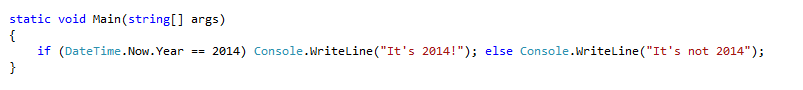
\includegraphics[width=6in]{figures/line_coverage.png}
	\end{center}
\caption{A valid program that is all on one line.}
\label{lineCoverage}
\end{figure}

An easy but non-ideal solution to this is to require that developers only place one statement on each line. Alternatively, a more complex coverage analysis tool could be used that takes this into account.

Statement coverage is the term used when talking about the number of program statements that are executed by testing \citep{Myers:2004:AST:983238}. \citet{Myers:2004:AST:983238} argue that statement coverage is `generally useless' as a metric of test quality because of the number of problems that it can potentially miss.

The example provided by \citet{Myers:2004:AST:983238} gives the code as shown in Figure \ref{codeCoverage}. They argue that a single test can provide 100\% statement coverage for the code by passing in the values \verb+A=2, B=0, X=3+, even though the code could be logically incorrect. The example that they provide is that if the first decision should be an \verb+or+ instead of an \verb+and+, then the single test will not notice, despite providing 100\% statement coverage.

\begin{figure}[h]
	\begin{center}
		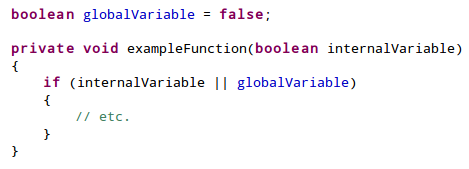
\includegraphics[width=2in]{figures/code_coverage.png}
	\end{center}
\caption{The sample code provided by \citet{Myers:2004:AST:983238}.}
\label{codeCoverage}
\end{figure}

Despite the flaws of statement coverage, it is popular because it quickly allows developers to see which parts of their code has gone completely untested. No great amount of calculation is required, so measurement and analysis should be quick to execute. For more a more thorough inspection of code coverage, branch coverage is now introduced.

\subsection{Branch Coverage}

\subsubsection{Control Flow Graph}

Before branch coverage can be introduced, the concept of a program control flow graph must be explained. A control flow graph shows the potential paths through a piece of code. Figure \ref{cfg} shows the control flow graph for the code listed in Figure \ref{codeCoverage}. At the top of the control flow graph is the entry point to the program. From there, the first conditional statement is represented as a vertex of the graph. From that vertex there are two outward arrows. One represents the case when the conditional statement evaluates to true, and the other to false \citep{Myers:2004:AST:983238}

\begin{figure}
\begin{minipage}{0.5\textwidth}
\centering
		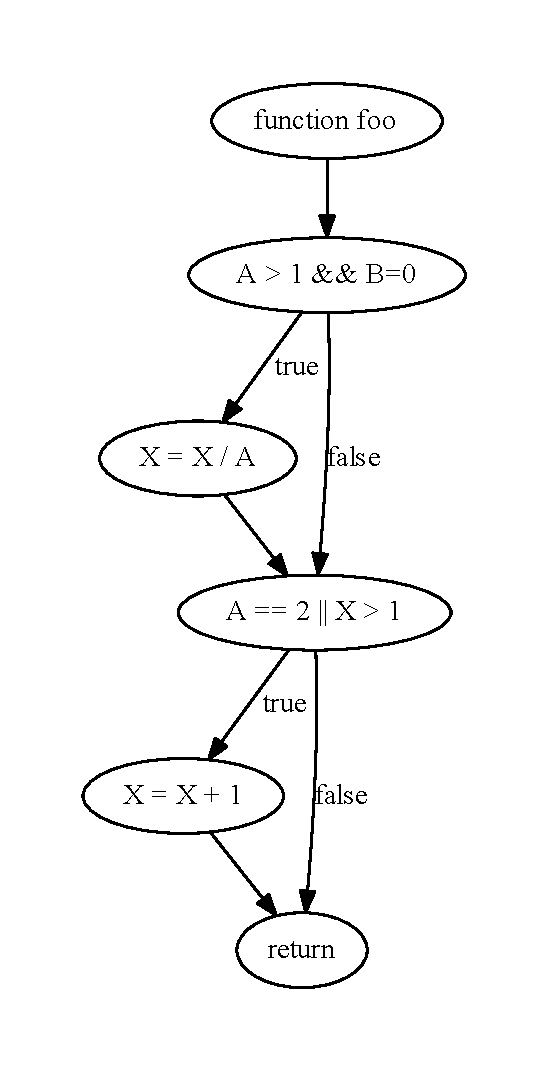
\includegraphics[scale=0.3]{figures/cfg.pdf}
\caption{A simple control flow graph for the function foo}
\label{cfg}
\end{minipage}
\begin{minipage}{0.49\textwidth}
\centering
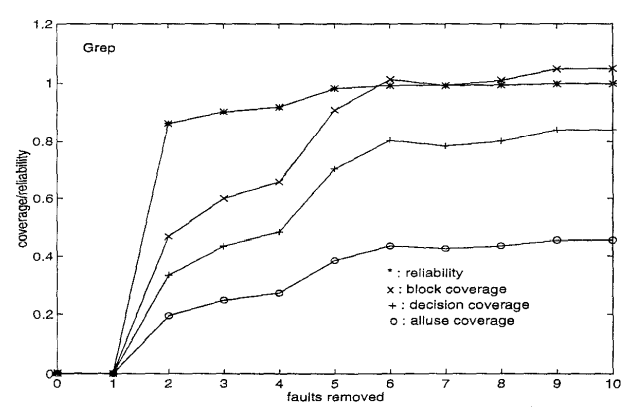
\includegraphics[width=3in]{figures/coverage_reliability.png}
\caption{\citet{497650}'s results of testing various coverage approaches on Grep}
\label{coverageReliability}
\end{minipage}
\end{figure}

\subsubsection{Branch Coverage}

There appears to some confusion between the terms `decision coverage' and `branch coverage'. Some sources state that decision coverage is a synonym for branch coverage \citep{softwareTestingBranchDecision, hitexBranchDecision}, but other sources explain that there is a subtle difference \citep{tmgBranchDecision, bullsEyeBranchDecision}. Branch coverage is explained as counting the number of edges of a control flow graph that have been executed, and comparing it with the total number of edges in the control flow graph. Decision coverage is explained as very similar, but only the edges coming from vertices that have more than one outbound edge are considered. From here onwards in the report I will refer to branch coverage, because it is only a minor implementation detail from my perspective.

In Figure \ref{cfg} there are two branching points - both of the conditional statements. For 100\% branch coverage it is necessary for every edge to have been executed at least once by the test set. An alternative way to think of this is that at every decision point in the program, the outcome of each decision has been executed at least once. At an \verb+if+ statement, the case where the outcome is true has been executed as well as the case where the outcome is false is said to have 100\% branch coverage. If branch coverage is 100\%, then so should statement coverage \citep{Myers:2004:AST:983238}.

However, \citet{Myers:2004:AST:983238} also argue that branch coverage can be a weak test quality metric. Going back to the code listed in Figure \ref{codeCoverage}, branch coverage can be satisfied with the two following test cases: \verb+A=2, B=0, X=1+ and \verb+A=3, B=1, X=1+. However, if the second conditional statement was supposed to check that X < 1 instead of X > 1, then this will not be picked up by any tests, despite the branch coverage being 100\%. \citet{497650} have done a comparison of the effectiveness of branch coverage and statement coverage after they inserted some random faults in the Unix utility Grep. Their results show in Figure \ref{coverageReliability} that block coverage analysis requires a higher percentage of coverage to find the same number of faults when compared to decision coverage.

\subsection{Path Coverage}

%Another approach to determining the quality of a test set is to consider the path coverage of the code being tested. A section of code can have many paths through it. In the sample code in figure \ref{sampleCoverageCode} there are two obvious paths. The first is through the if statement, the second is to skip the if statement. For a section of code with $n$ inputs, there are potentially $2^n$ code paths \cite{something}. This can of course be problematic, because for any program larger than a few lines of code the numbers of code paths will be very large, quickly getting to the point where it is not feasible to compute all paths, and therefore not possible to check if all paths are covered by a test set.

\begin{figure}%
    \centering
    \subfloat[Path 1]{{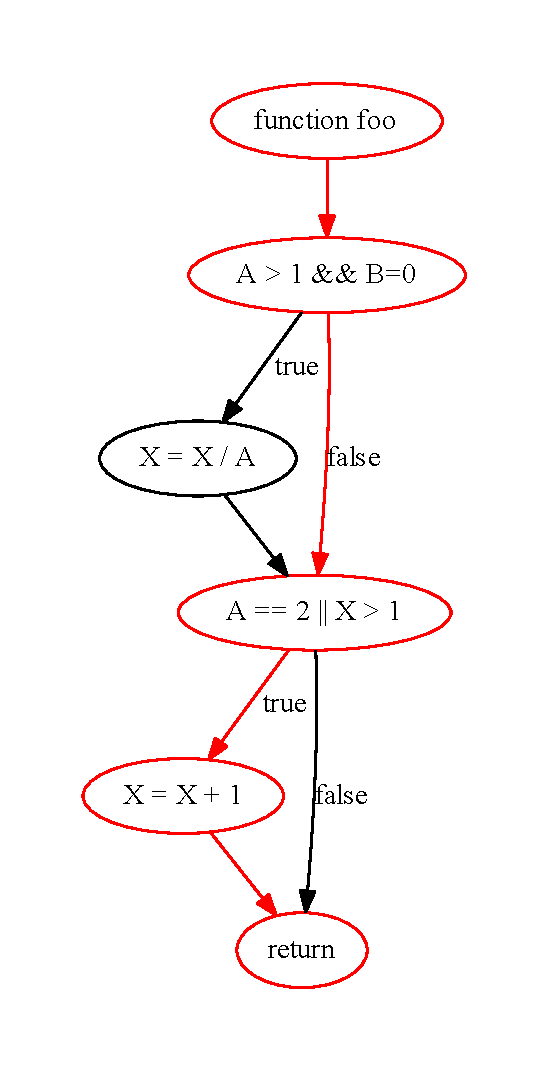
\includegraphics[scale=0.25]{figures/cfg_path1.pdf} }}%
    \qquad
    \subfloat[Path 2]{{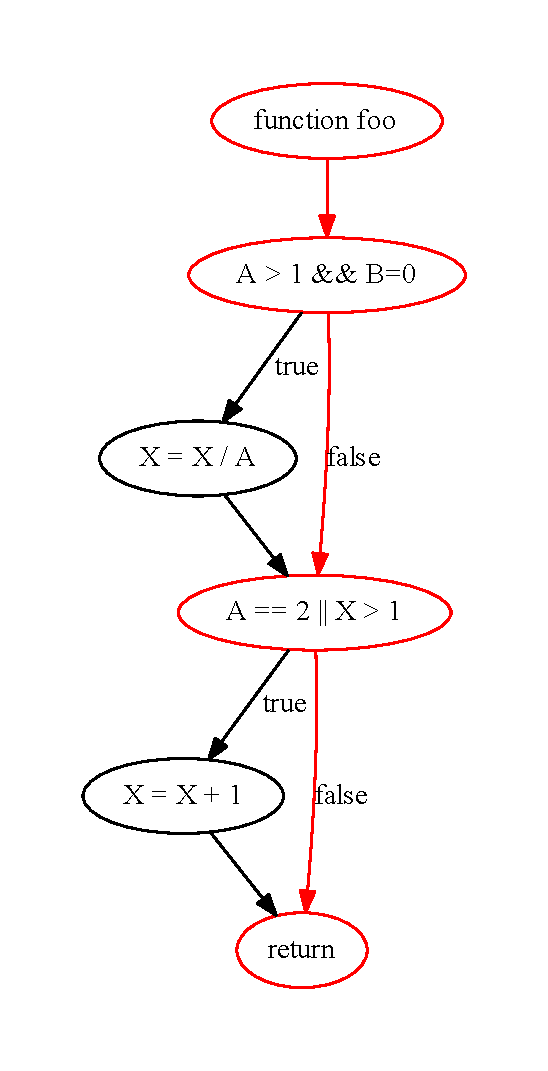
\includegraphics[scale=0.25]{figures/cfg_path2.pdf} }}%
    \qquad
    \subfloat[Path 3]{{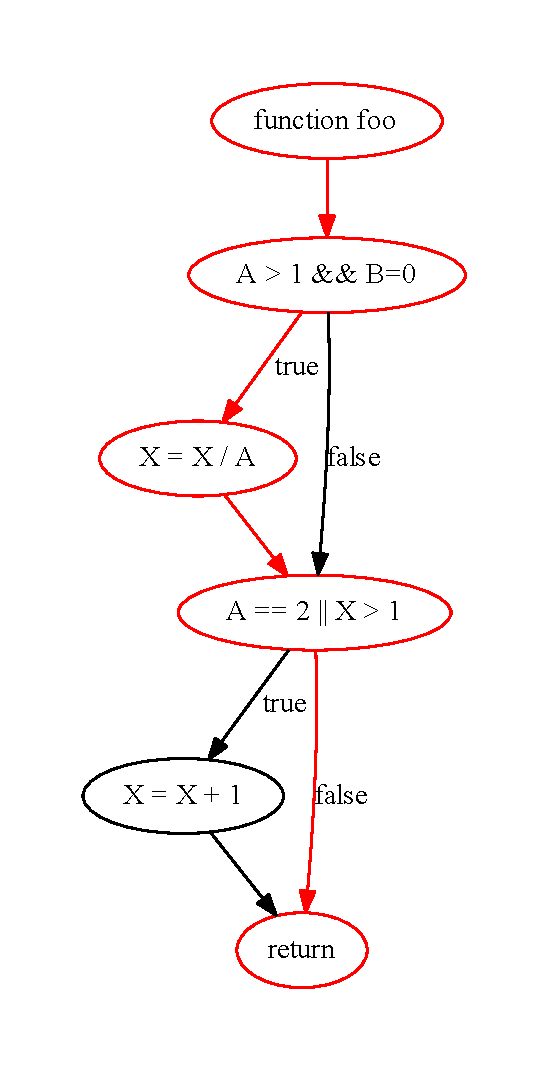
\includegraphics[scale=0.25]{figures/cfg_path3.pdf} }}%
    \qquad
    \subfloat[Path 4]{{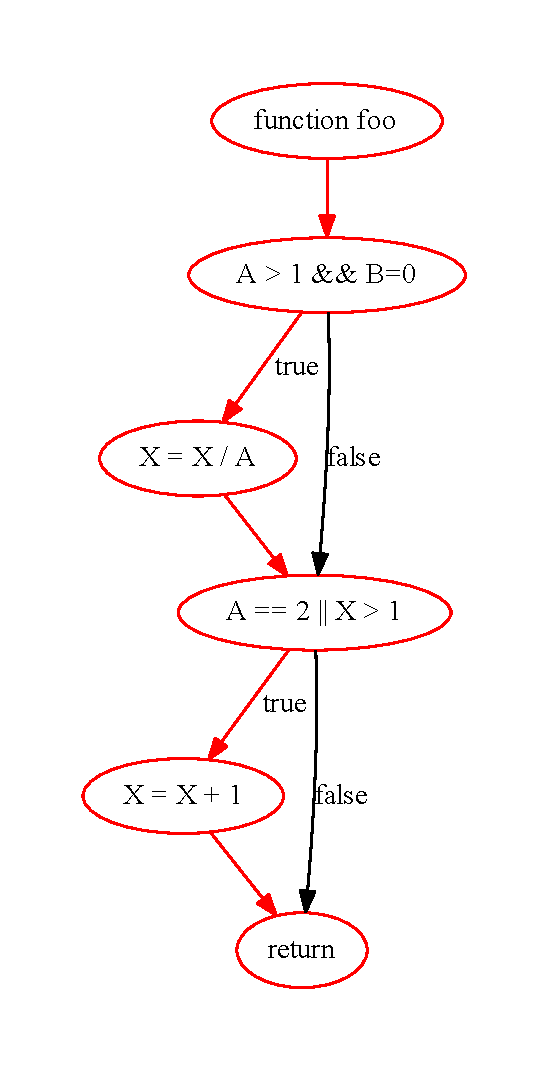
\includegraphics[scale=0.25]{figures/cfg_path4.pdf} }}%
    \caption{The possible paths through the program}%
    \label{programPaths}%
\end{figure}

Path coverage is a stronger test quality metric. Branch coverage covers all possible decisions at a program branch, but path coverage considers every possible path through the program \citep{Myers:2004:AST:983238, softwareTestingIntro}. Using the example again given by \citet{Myers:2004:AST:983238} in Figure \ref{codeCoverage}, there are four possible paths through the code. Each \verb+if+ statement can evaluate to true or false. Every path through the program therefore is when the \verb+if+ statements evaluate as follows: \verb+false, true+, \verb+false, false+, \verb+true, false+ and \verb+true, true+. Figure \ref{programPaths} colours in red the possible paths through the program.

Because \verb+if+ statements only have two possible outcomes - true or false - the number of paths through a program that only contains $n$ sequential \verb+if+ decisions is $2^n$. However, the complexity is increased with statements such as \verb+switch+ that can have any number of paths. This is known as the cyclomatic complexity of the program, and the calculation to calculate this complexity from a control flow graph was given by \citet{1702388}:

\begin{equation}
M = E - N + 2P
\end{equation}

Where M is the cyclomatic complexity, E is the number of edges in the graph, N is the number of nodes in the graph and P is the number of exit nodes. With this formula we can verify that the number of paths through the code in Figure \ref{codeCoverage} is 4. There are 7 edges, 5 nodes, and one exit point (the return statement).

\begin{equation}
M = 7 - 5 + (2*1)
\end{equation}

\citet{Myers:2004:AST:983238} are even more critical of path coverage than the previous test quality metrics described. Their main points of criticism are:

\begin{enumerate}
\item The time that it would take to even generate all possible paths through a program grows exponentially with the number of branches in the program.
\item As some decisions are dependent on the outcome of previous decisions, once all possible paths have been generated it is then necessary to do further computation to calculate the actual number of possible paths through the code.
\item Even with each possible path through the code covered, there is no guarantee that the inputs used by the tests will find every problem with the code.
\end{enumerate}

In her early work on the effectiveness of path analysis, \citet{1658851} found that while the data used by tests will cause path coverage to be completed, it may not actually find bugs that are present.  therefore recommends that tests that have good path coverage are used in conjunction with boundary input data tests.

\subsection{Mutation Testing}

Mutation testing is another approach to determining the quality of a test set. Consider the following statement:

\begin{lstlisting}
y := 3x + 4 - z;
\end{lstlisting}

This is the fragment of code that we want to check that our test sets sufficiently cover. The code is called the \emph{ground string}. From the ground string, mutant strings are created. These mutant strings are based on the ground string, but have been `mutated' in some way such that they are not the same as the ground string, but still compile \citep{softwareTestingIntro}. Some example mutants might be:

\begin{lstlisting}
y := 3x - 4 - z;
y := 3x - 4 + z;
y := 10x + 6 - i;
\end{lstlisting}

The mutants all compile, but alter the outcome of executing the function. So the quality of a test set can be determined by running the set on each of the mutants and checking how many of the mutants are rejected. The perfect test set would reject all of the mutants \citep{softwareTestingIntro}. The example above is greatly simplified, and in reality it is unlikely that all of the mutants would be caught by the test set.

According to \citet{softwareTestingIntro}, in addition to being used to determine the quality of test sets, mutation testing (and path coverage and code coverage) can be used to help develop a high quality test set. He claims that there are 11 mutation operations that should be used, regardless of the programming language in question:

\begin{description}
\item[ABS] Absolute Value Insertion - Forces the tester to have at least one positive, one 0 and one negative value for the variable that has the \verb+abs+ function applied to it.
\item[AOR] Arithmetic Operator Replacement - Swapping between addition, subtraction, multiplication, division and modulus operators.
\item[ROR] Relational Operator Replacement - $<, \leq, ==, \geq, >, \neq$ operators are interchanged.
\item[COR] Conditional Operator Replacement - AND, OR, true and false are interchanged.
\item [SOR] Shift Operator Replacement - The shift operators $<<, >> $and $>>>$ are interchanged.
\item[LOR] Logical Operator Replacement - Bitwise operators AND (\&), OR ($\mid$) and exclusive OR (\^{}).
\item[ASR] Assignment Operator Replacement - The operators $+=, -=, *=, /=, \%=, \&=, |=, $\^{}$=, <<=, >>=, >>>=$ are replaced with one of the other operators.
\item[UOI] Unary Operator Insertion - One of the unary operators $+, -, !, ~ $ is inserted in a valid position.
\item[UOD] Unary Operator Deletion - One of the unary operators $+, -, !, ~ $ is deleted from a position where a deletion will leave the statement valid.
\item[SVR] Scalar Variable Replacement - Each reference to a variable is replaced by another variable in scope of an appropriate type.
\item[BSR] Bomb Statement Replacement - Each statement is replaced by a bomb statement that causes the program to fail.
\end{description}

\subsection{Coverage Analysis Software}

There are numerous tools that can assist in calculating coverage metrics for a test suite. A selection of these are detailed in this section, and their general features will be taken into consideration during the design phase of this project.

\subsubsection{JaCoCo}

JaCoCo is a free Java code coverage library that works with Java 7 and 8 \cite{JaCoCo}. The library can be used to record statement and branch coverage of executed Java code, and will then produce a report in HTML, CSV or XML format. It provides a public API and thorough documentation with the intention that plugins make use of it for measuring coverage.

\subsubsection{EclEmma}

\begin{figure}
\begin{minipage}[b]{0.44\textwidth}
\centering
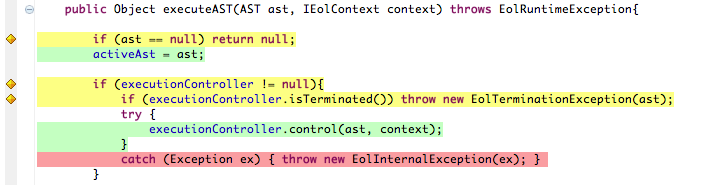
\includegraphics[width=0.9\linewidth]{figures/EclEmma}
\end{minipage}
\begin{minipage}[b]{0.1\textwidth}
\vspace{3.00mm}
\end{minipage}
\begin{minipage}[b]{0.44\textwidth}
\centering
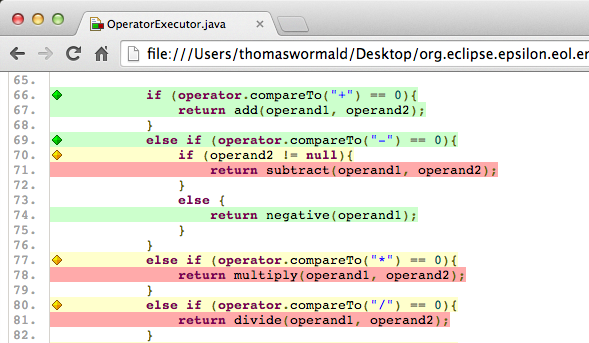
\includegraphics[width=0.9\linewidth]{figures/EclEmmaHTML}
\end{minipage}
\caption{Left: EclEmma as an Eclipse plugin. Right: Output of EclEmma in HTML format}
\label{fig:eclemma}
\end{figure}

EclEmma is an Eclipse plugin that uses JaCoCo \cite{EclEmma}, and was developed alongside JaCoCo by the same developers. As shown in Figure \ref{fig:eclemma} it highlights executed code in green, branches that have been partially executed in yellow, and non-executed code in red. To the left of the yellow statements is an icon, which when hovered over with the mouse tells the user how many branches there are in total, and how many of those branches were executed.

EclEmma can also export coverage reports to various formats. One option is a HTML document, as shown in Figure \ref{fig:eclemma}.

\subsubsection{NCover}

NCover is a suite of commercial code coverage tools written for use with .NET \citep{NCover}. Like EclEmma, NCover offers an IDE plugin tool (for Visual Studio) that will highlight code statements to indicate the level of coverage of unit tests. NCover can output reports to HTML, and there is also a standalone desktop application that provides an `interactive view of your coverage data so you can reduce errors, keep down your costs and deliver applications on-time' \citep{NCover}. 

\subsubsection{dotCover}

dotCover is another .NET code coverage tool \cite{dotCover}. It is quite significantly cheaper than NCover, but offers many of the same features, including full Visual Studio integration and output to HTML, XML and JSON reports. However, the only method of coverage analysis that it offers is statement coverage, which as discussed before is not a particularly strong form of coverage.

Some of the common features across all of these tools that should be considered in any tools that I implement are IDE integration, syntax highlighting and generated reports that include syntax highlighting and statistics about coverage levels.
\section{Conclusion}

This literature review has introduced the concepts that are necessary for this project. Where appropriate it has compared and contrasted information from various sources. The introduction of model driven engineering has given some context about the project, and the helped to justify the reason for continuing to develop MDE tools. The second half of the literature review has looked at test coverage, looking at some of the different types of coverage and the tools that can be used to analyse coverage.